\documentclass[12pt,a4paper]{article}
\usepackage[utf8]{inputenc}
\usepackage[spanish]{babel}
\usepackage{graphicx}
\usepackage{geometry}
\usepackage{hyperref}
\usepackage{tikz}
\geometry{top=2.5cm, bottom=2.5cm, left=2.5cm, right=2.5cm}

\begin{document}
\begin{center}

\includegraphics[width=0.4\textwidth]{LOGO_RAS.png} \\
\vspace{1cm}
{\LARGE \textbf{Bases de Competencia: Velocistas Open}} \\
\vspace{0.5cm}
{\large \textbf{Universidad de Concepción - RAS UdeC}} \\
{\large \textbf{4 de diciembre de 2026}} \\
\end{center}
\vspace{1cm}

\noindent\textit{Basado en la categoría Robotrace del torneo All Japan Micromouse Contest y en la categoría Velocidad de la Competencia Robótica UTFSM.}

\section*{Objetivo de la Competencia}
El objetivo de la competencia es recorrer un circuito en el menor tiempo posible utilizando un robot seguidor de lneas autónomo. Un robot que participa en esta competencia se denomina `Velocista''.

\section*{Categoría Open (Abierta)}
Esta categoría es abierta a todo público, sin restricción de ser estudiante universitario. Se podrán inscribir equipos de 2 o 3 personas.

\section*{Inscripción}
Las inscripciones estarán abiertas hasta el \textbf{22 de noviembre a las 23:59 hrs}.

La inscripción y la participación son gratuitas. No se requiere pago ni comprobante.

\section*{Reglas de la Competencia}
\begin{itemize}
    \item Una ronda consiste en el paso de todos los Velocistas participantes por la pista.
    \item En una ronda, cada equipo competidor tiene 9 minutos para un máximo de 3 intentos de vuelta.
    \item La proyección del Velocista con respecto al escenario debe cubrir la línea del trayecto. Si el Velocista se sale completamente se considerará como vuelta inválida.
    \item Al terminar el recorrido, el Velocista debe detenerse automáticamente en el área de Salida-Meta por al menos 2 segundos.
    \item La vuelta más rápida será registrada como el tiempo oficial.
    \item El equipo que logre el tiempo más rápido en la última ronda, será el ganador.
\end{itemize}

\section*{Reglas del Velocista}
\begin{itemize}
    \item El Velocista debe ser autónomo durante su participación.
    \item El tamaño del Velocista no puede exceder un largo de 25 [cm], ancho de 25 [cm] y alto de 20 [cm].
    \item El Velocista no puede estar equipado con ningún mecanismo de sujeción que pudiera generar daños en la pista.
\end{itemize}

\section*{Reglas de la Pista}
\begin{itemize}
    \item La superficie del escenario está hecha de tableros negros.
    \item Las líneas del recorrido están hechas con cinta blanca de 19 [mm] de ancho.
    \item El recorrido de la pista será secreto hasta el primer día de competencia.
\end{itemize}


\section*{Esquemas de la Pista (Referencia Robotracer)}
A continuación se presentan las figuras de referencia y sus explicaciones, extraídas del reglamento oficial de la categoría Robotracer:

\begin{figure}[h!]
    \centering
    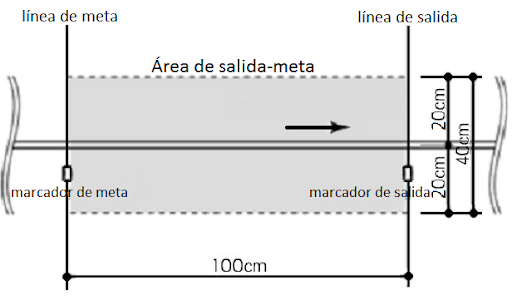
\includegraphics[width=0.6\textwidth]{cropped-unnamed-3.png}
    \caption{\textbf{Intersección en 90 grados:} Cuando las líneas se crucen, el ángulo de cruce será de 90 grados $\pm 5$ grados. 10 cm antes y después del punto de intersección de las líneas, las líneas serán rectas.}
\end{figure}

\begin{figure}[h!]
    \centering
    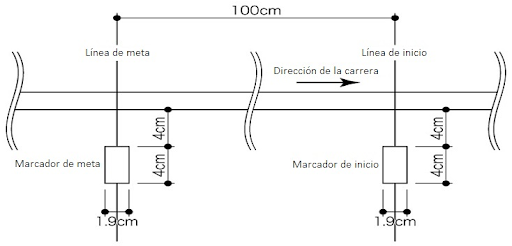
\includegraphics[width=0.6\textwidth]{cropped-unnamed.png}
    \caption{\textbf{Zona de meta y marcas (hits):} La zona de meta estará delimitada por dos marcas (hits) ubicadas a la derecha del sentido de la carrera, separadas por 1 metro. Antes de la meta, y después de la salida, el tramo será recto.}
\end{figure}

\begin{figure}[h!]
    \centering
    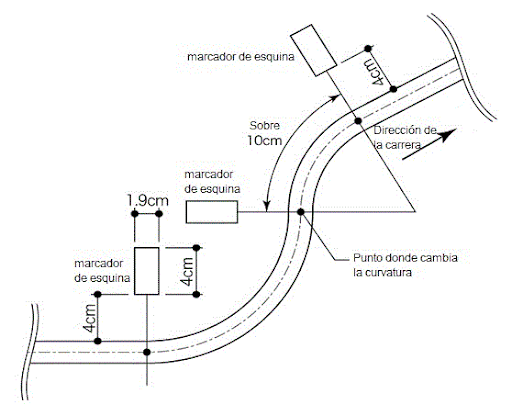
\includegraphics[width=0.6\textwidth]{unnamed-2.png}
    \caption{\textbf{Marca lateral de curva:} En cada cambio de curvatura habrá una marca lateral a la izquierda. Los marcadores de esquina no se superponen con otros marcadores de esquina.}
\end{figure}

\begin{figure}[h!]
    \centering
    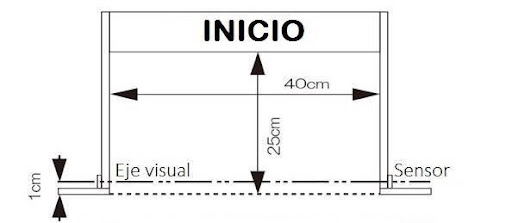
\includegraphics[width=0.4\textwidth]{unnamed-3.jpg}
    \caption{\textbf{Ubicación de los sensores:} Los lugares donde se ubican los sensores de inicio y final están indicados en la figura. Estos son del tipo infrarrojo y su eje óptico se ubica 1 [cm] por encima del piso.}
\end{figure}

\vspace{1cm}
\noindent El equipo organizador se reserva el derecho a modificar las bases y reglas de la competencia. En tal caso, se informará a los equipos inscritos.
\end{document}
